\newpage
\section{Spezifikation}
Basierend auf dem entwickelten Konzept und den definierten Anforderungen wird die detaillierte Spezifikation des Systems ausgearbeitet. Diese umfasst die Architektur des gesamten Systems, welche die Aufteilung in einzelne Komponenten und deren Interaktion untereinander beschreibt. Ebenso wurden die Schnittstellen zwischen den Komponenten definiert. Weiterhin wird erläutert, wie das System mit seiner Umgebung interagiert. Die technische Spezifikation umfasst die verwendete Hardware sowie die eingesetzten Protokolle und Standards, die für Umsetzung der einzelnen Komponenten benötigt werden.

\subsection{Architektur}
\begin{itemize}
    \item Systemarchitektur: Gesamtdarstellung des Systems, wie Komponenten zusammenarbeiten
    \item Unterteilung in 3 Komponenten (Audio, User Interface, NN)
    \item Hier SA/RT Kontextdiagramm (evtl. ein Gesamt-Diagramm und pro Komponente ein weiteres)
    \item Hier SA/RT Modell für Zustandsautomat? und ggf. weitere Modelle
    
    \begin{figure}[H]
    	\centering
    	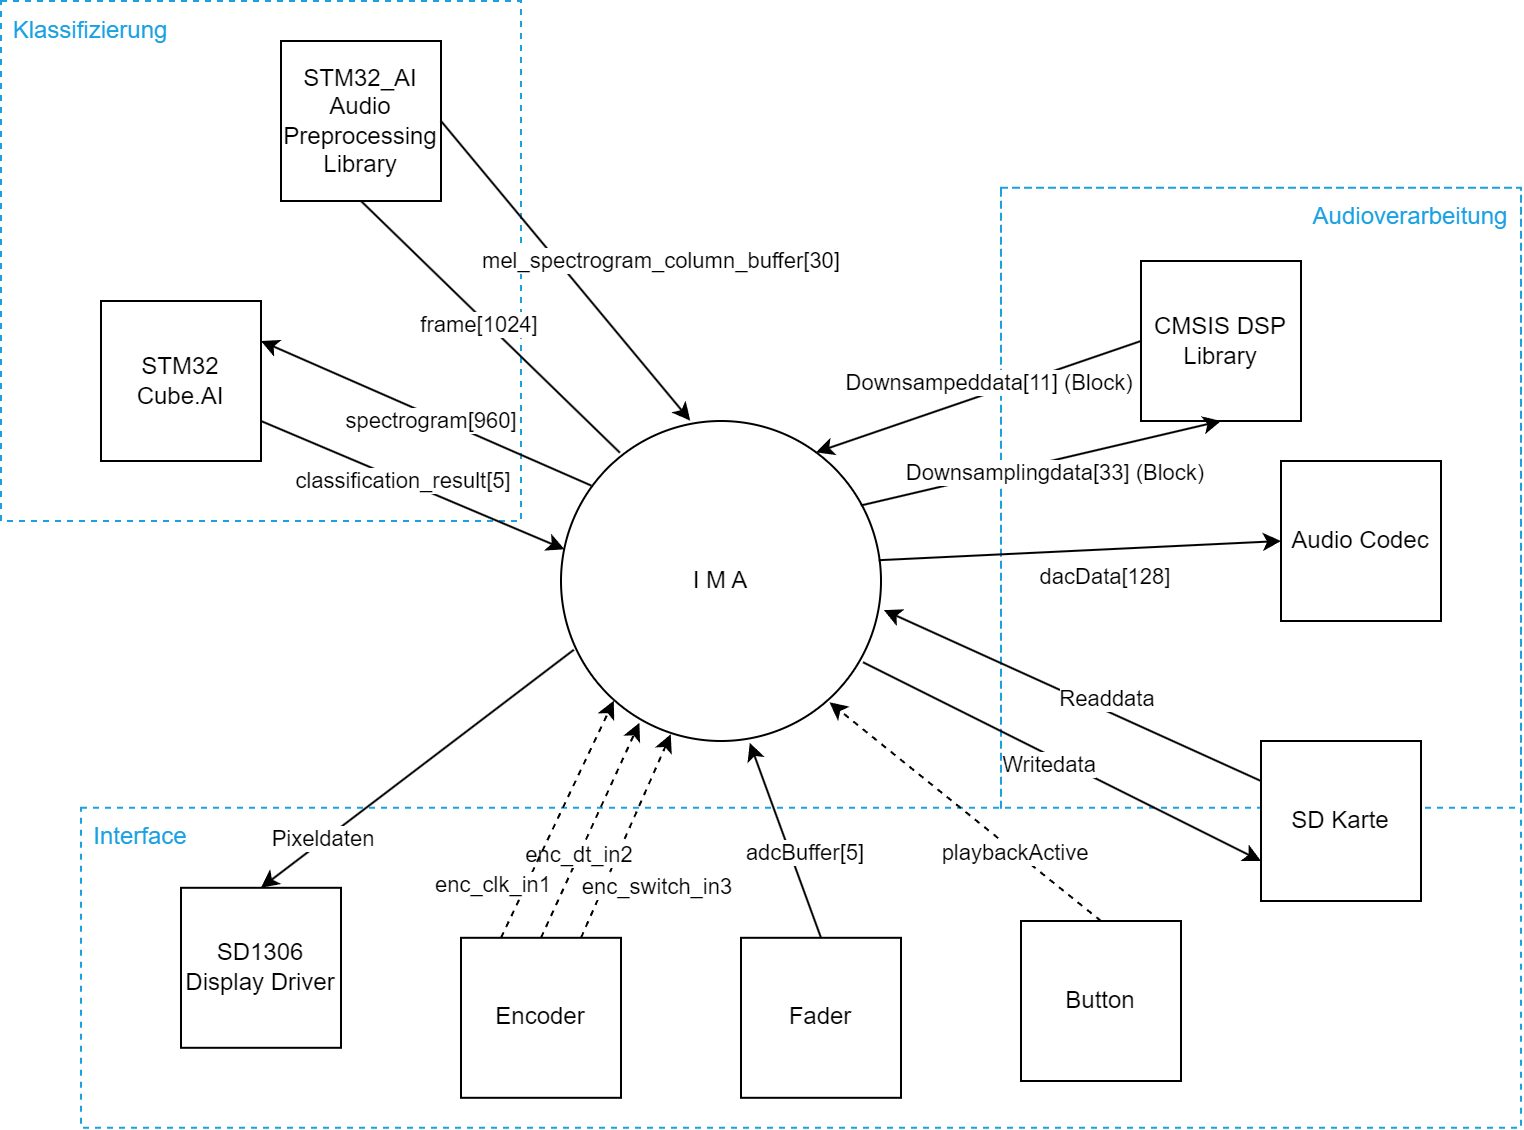
\includegraphics[width=0.8\textwidth]{images/04_spezifikation/kontextdiagramm_gesamt.drawio.png}
    	\caption{Kontextdiagramm des Gesamtsystems}
    	\label{fig:context_diagram_gesamt}
    \end{figure}
    
    %TODO: ausformulieren
    
    %TODO: Kontextdiagramme pro Untersystem
   
    
    \begin{figure}[H]
    	\centering
    	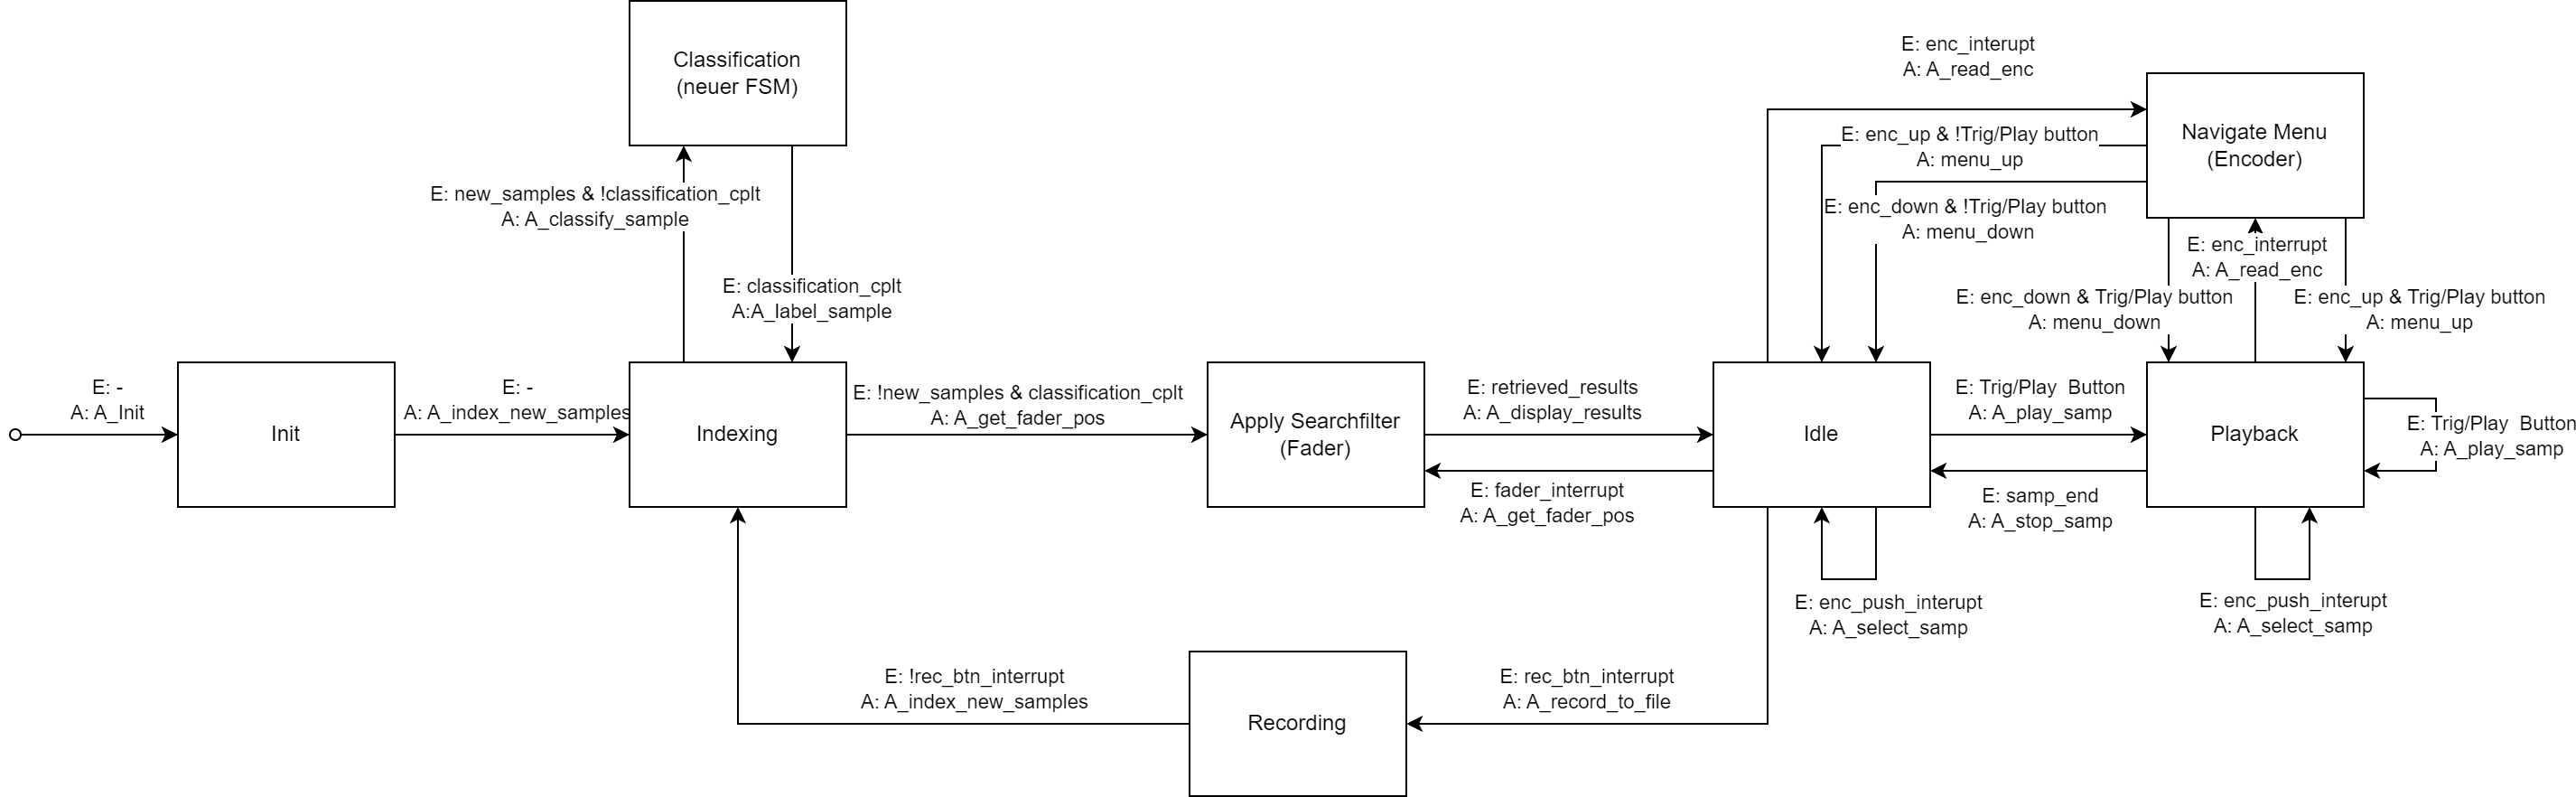
\includegraphics[width=1.0\textwidth]{images/04_spezifikation/fsm.drawio.png}
    	\caption{Zustandsautomat des Systems}
    	\label{fig:fsm}
    \end{figure}
    
    Folgendes Diagramm zeigt die Relation und Interaktion der 4 Komponenten miteinander.
    
    \begin{figure}[H]
    	\centering
    	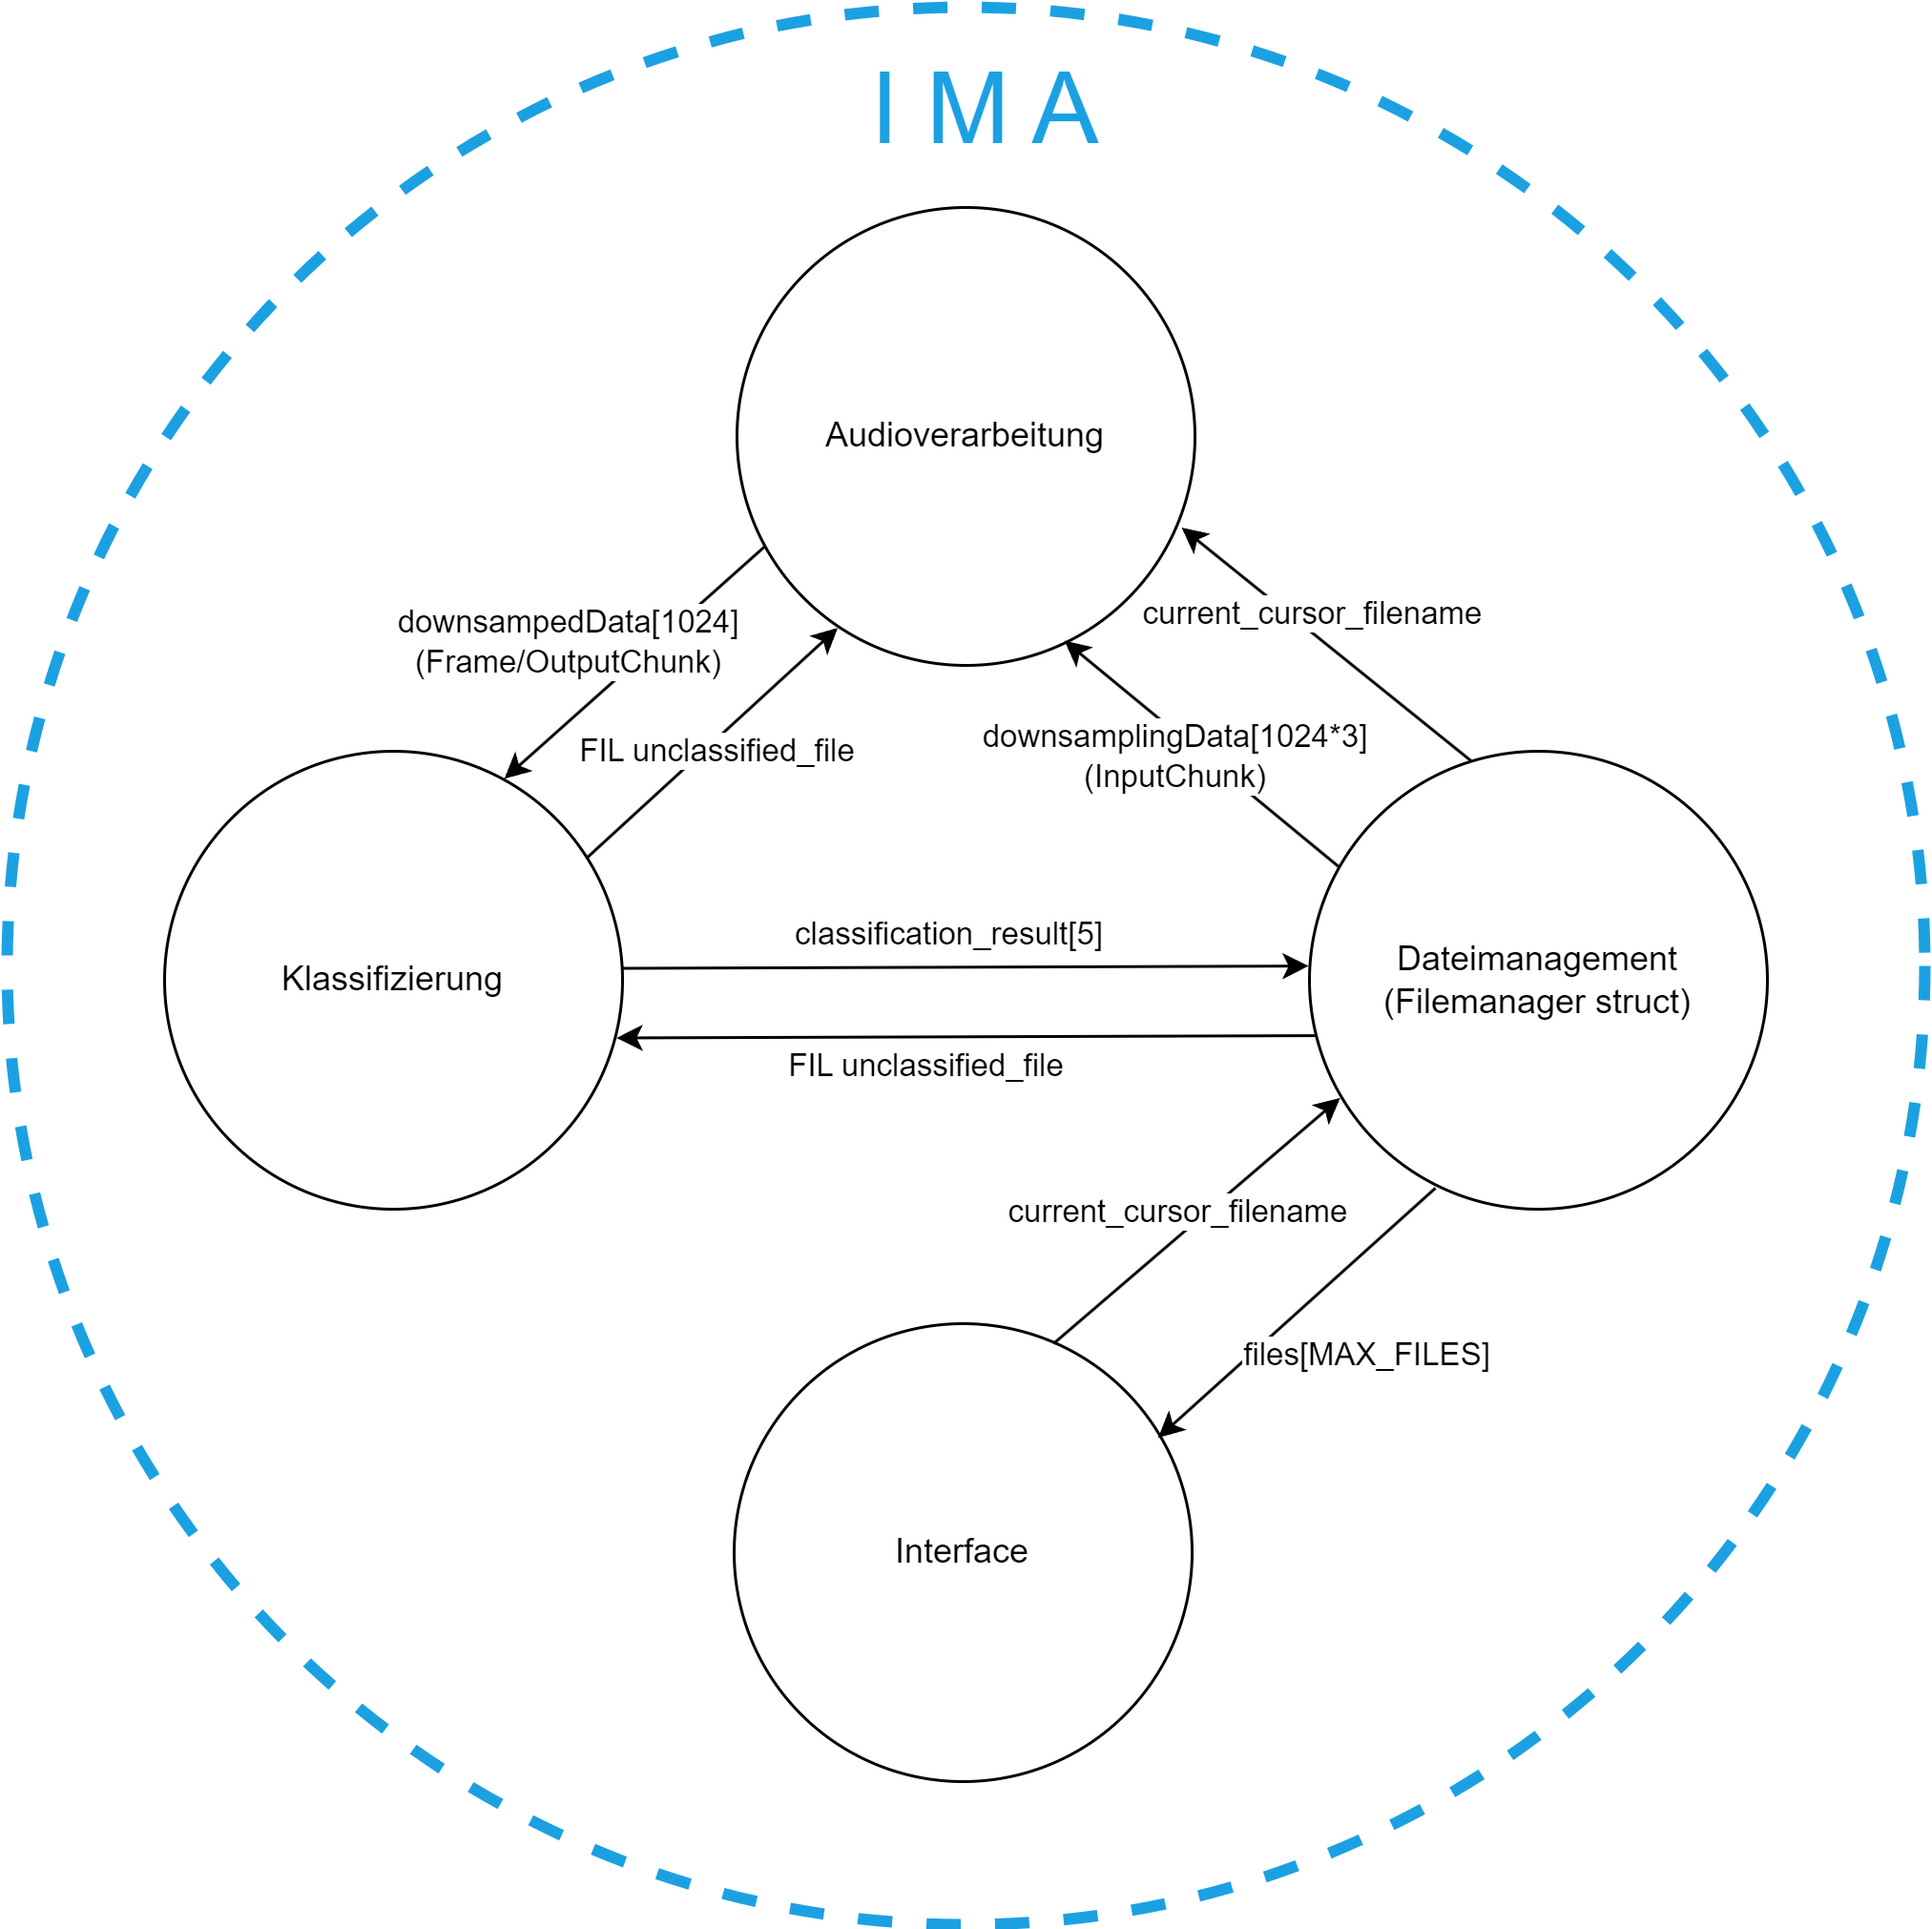
\includegraphics[width=1.0\textwidth]{images/04_spezifikation/komponentendiagramm.drawio.png}
    	\caption{Komponentendiagramm}
    	\label{fig:komponentendiagramm}
    \end{figure}
\end{itemize}